\RequirePackage{fix-cm}
\documentclass[smallextended,final]{svjour3}       % onecolumn (second format)
\smartqed  % flush right qed marks, e.g. at end of proof
\usepackage{graphicx}
%
% \usepackage{mathptmx}      % use Times fonts if available on your TeX system
%
% insert here the call for the packages your document requires
%\usepackage{latexsym}
\usepackage{tikz}     % For adding axes to plots
\usetikzlibrary{positioning}
\usepackage{graphicx} % For including PDFs
\usepackage{amsmath} % assumes amsmath package installed
\usepackage{amssymb}  % assumes amsmath package installed
\usepackage{booktabs} % For formal tables
\usepackage[colorlinks,allcolors=blue]{hyperref}

%
% please place your own definitions here and don't use \def but
% \newcommand{}{}

%% Command for creating multiplie-line cells inside a table environment
\newcommand{\multilinecell}[2][c]{%
  \begin{tabular}[#1]{@{}c@{}}#2\end{tabular}}

%% Create a ``Lemma'' environment that does not have italics font.
\spnewtheorem{plainlemma}{Lemma}{\bf}{}
%% Create a ``Theorem'' environment that is not numbered.
\spnewtheorem*{onetheorem}{Theorem}{\bf}{}
\spnewtheorem*{proofdot}{Proof.}{\it}{}

%% \newcommand{\Bigl}{\mathopen\Big}
%% \newcommand{\Bigr}{\mathclose\Big}
%
% Insert the name of "your journal" with
\journalname{Numerical Algorithms}
%
\begin{document}

\title{Interpolation of Sparse High-Dimensional Data\thanks
  {This work was supported by the National Science Foundation Grant CNS-1565314.}
}
% \subtitle{Do you have a subtitle?\\ If so, write it here}

%\titlerunning{Short form of title}        % if too long for running head

\author{Thomas C. H. Lux   \and
  Layne T. Watson          \and
  Tyler H. Chang           \and
  Yili Hong                \and
  Kirk Cameron
}

%\authorrunning{Short form of author list} % if too long for running head

\institute{Thomas Lux \at
  Virginia Polytechnic Institute \& State University (VPI\&SU) \\
  Blacksburg, VA 24061 \\
  \email{tchlux@vt.edu}
}

\date{Received: date / Accepted: date}
% The correct dates will be entered by the editor

\maketitle

\begin{abstract}
A rapid increase in the quantity of data available is allowing all fields of science to generate more accurate models of multivariate phenomena. Regression and interpolation become challenging when the dimension of data is large, especially while maintaining tractable computational complexity. While regression is a popular approach to solving approximation problems with high dimension, there are often advantages to interpolation. This paper presents error bounds for interpolants on moderately high dimensional problems and contrasts their performance with that of popular regression techniques. Empirical results demonstrate the viability of interpolants for high dimensional approximation problems, suggesting that these techniques are capable of effectively modeling multivariate phenomena while maintaining flexibility in different application domains.

\keywords{approximation \and regression \and interpolation \and high dimension \and error bound}
% \PACS{PACS code1 \and PACS code2 \and more}
% \subclass{MSC code1 \and MSC code2 \and more}
\end{abstract}

%     Introduction     
%======================

%% ===================================================================
\section{Introduction}
\label{sec:introduction}

Regression and interpolation are problems of considerable importance that find applications across many fields of science. Pollution and air quality analysis \cite{de2008field}, energy consumption management \cite{lazos2014optimisation}, and student performance prediction \cite{cortez2008using,lux2016applications} are a few of many interdisciplinary applications of multivariate regression for predictive analysis. As discussed later, these techniques can also be applied to prediction problems related to forest fire risk assessment \cite{cortez2007data}, Parkinson's patient clinical evaluations \cite{tsanas2010accurate}, local rainfall and weather \cite{williams2009rattle}, credit card transactions \cite{pozzolo2015calibrating}, and high performance computing (HPC) file input/output (I/O) \cite{lux2018nonparametric}.

Regression and interpolation have a considerable theoretical base in one dimension \cite{cheney2009course}. Splines in particular are well understood as an interpolation technique in one dimension \cite{de1978practical}, particularly B-splines. Tensor products of B-splines \cite{unther1996interpolating} or other basis functions have an unfortunate exponential scaling with increasing dimension. Exponential scaling prohibits tensor products from being reasonably applied beyond three-dimensional data. In order to address this dimensional scaling challenge, C. de Boor and others proposed box splines \cite{de2013box}, of which one of the approximation techniques in this work is composed \cite{lux2018novel}.

The theoretical foundation of low dimensional interpolation allows the construction of strong error bounds that are absent from high dimensional problems. This work extends some known results regarding the secant method \cite{dennis1996numerical} to construct an interpolation error bound for problems of arbitrary dimension. These error bounds are useful, considering the same cannot be said for regression algorithms in general. The maximum complexity of an interpolant is bounded by the amount of data available, while the maximum complexity of a regressor is bounded by both the amount of data and the chosen parametric form. For this reason, generic uniform bounds are largely unobtainable for regression techniques on arbitrary approximation problems, even when the approximation domain is bounded.

Aside from theoretical motivation for the use of interpolants, there are often computational advantages as well. Interpolants do not have the need for \textit{fitting} data, or minimizing error with respect to model parameters. In applications where the amount of data is large and the relative number of predictions that need to be made for a given collection of data is small, the direct application of an interpolant is much less computationally expensive.

In this work, multivariate interpolation is defined given a closed convex subset $Y$ of a metrizable topological vector space with metric $s$, some function $f:\mathbb{R}^d \rightarrow Y$ and a set of points $X = \bigl\{x^{(1)}$,$\ldots$,$x^{(n)}\bigr\} \subset \mathbb{R}^d,$ along with associated function values $f\bigl(x^{(i)}\bigr)$. The goal is to construct an approximation $\hat f: \mathbb{R}^d \rightarrow Y$ such that $\hat f\bigl(x^{(i)}\bigr) = f\bigl(x^{(i)}\bigr)$ for all $i = 1$,$\ldots$,$n$. It is often the case that the form of the true underlying function $f$ is unknown, however it is still desirable to construct an approximation $\hat f$ with small approximation error at $y \notin X$. The two metric spaces that will be discussed in this work are the real numbers with metric $s(x,y) = |x-y|$, and the set of cumulative distribution functions (CDFs) with the Kolmogorov-Smirnov (KS) statistic as metric.

Multivariate regression is often used when the underlying function is presumed to be stochastic, or stochastic error is introduced in the evaluation of $f$. Hence, multivariate regression relaxes the conditions of interpolation by choosing parameters $P$ defining $\hat f(x;P)$ to minimize the error vector $\Bigl( \bigl | \hat f \bigl(x^{(1)};P\bigr) - f\bigl(x^{(1)}\bigr) \bigr|$, $\ldots$, $\bigl | \hat f \bigl(x^{(n)}; P\bigr) - f\bigl(x^{(n)}\bigr) \bigr | \Bigr)$ in some norm. The difficult question in the case of regression is often what parametric form to adopt for any given application.

The most challenging problem when scaling in dimension is that the number of possible interactions between dimensions grows exponentially. Quantifying all possible interactions becomes intractable and hence beyond three-dimensional data, mostly linear models are used. That is not to say nonlinear models are absent, but nonlinearities are often either preconceived or model pairwise interactions between dimensions at most. Even globally nonlinear approximations such as neural networks are constructed from compositions of summed low-interaction functions \cite{clevert2015fast}.

Provided the theoretical and practical motivations for exploring interpolants, this work aims to study the empirical performance differences between a set of scalable (moderately) interpolation techniques and a set of common regression techniques. These techniques are applied to a collection of moderately high dimensional problems ($5 \le d \le 30$) and the empirical results are discussed.

The remainder of this paper is organized as follows. Sections \ref{sec:regression} and \ref{sec:interpolation} present the multivariate models. Section \ref{sec:error} presents the error measuring methodology that is used for collecting empirical results. Section \ref{sec:theory} presents the theoretical error bounds for interpolation. Section \ref{sec:data} presents the data sets for empirical approximation analysis and presents the approximation results for all models on these data sets. Section \ref{sec:discussion} analyzes and discusses the results, their implications, and their limitations. Finally, Section \ref{sec:conclusion} concludes.

% Art is a subjective form of personal expression and computers are
% just robots that are going to take over the world. \textit{*deep
% breath*} In order to communicate my frustration with the
% technological and information revolution, I'm going to write the
% rest of this paper in poetry.

% Star light, star bright \ldots

%% ===================================================================
\section{Multivariate Regression}
\label{sec:regression}
Multivariate regressors are capable of accurately modeling a complex dependence of a response (in $Y$) on multiple variables (represented as a points in $\mathbb{R}^{d}$). The approximations to some (unknown) underlying function $f: \mathbb{R}^d \rightarrow Y$ are chosen to minimize some error measure related to data samples $f\bigl(x^{(i)}\bigr)$. For example, least squares regression uses the sum of squared differences between modeled function values and true function values as an error measure. In this section and the next, some techniques are limited to approximating real valued functions ($Y \subset \mathbb{R}$). These techniques can be extended to real vector-valued ranges by repeating the construction for each component of the vector output. Throughout the following, $x$ denotes a $d$-tuple, $x_i$ the $i$th component of $x$, and $x^{(i)}$ the $i$th $d$-tuple data point. Different symbols are used to represent the approximation function $\hat f$.

\subsection{Multivariate Adaptive Regression Splines}
\label{sec:mars}
This approximation was introduced in \cite{friedman1991multivariate} and subsequently improved to its current version in \cite{stanford1993fast}, called fast multivariate adaptive regression splines (Fast MARS).In Fast MARS, a least squares fit model is iteratively built by beginning with a single constant valued function and adding two new basis functions at each iteration of the form
\begin{align*}
  B_{2j-1}(x) &= B_l(x) \bigl(x_i-x^{(p)}_i\bigr)_+, \\
  B_{2j}(x) &= B_k(x) \bigl(x_i-x^{(p)}_i\bigr)_- ,
\end{align*}
where $j$ is the iteration number, $1 \le p \le n$, and $B_l(x)$, $B_k(x)$ are basis functions from the previous iteration,
$$w_+ = \begin{cases} w, & w \geq 0 \\ 0, & w < 0 \end{cases},$$
and $w_- = (-w)_+$. After iteratively constructing a model, MARS then iteratively removes basis functions that do not contribute to goodness of fit. In effect, MARS creates a locally component-wise tensor product approximation of the data. The overall computational complexity of Fast MARS is $\mathcal{O}(n d m^3)$ where $m$ is the maximum number of underlying basis functions. This paper uses an implementation of Fast MARS \cite{rudy2017pyearth} with $m = 200$ throughout all experiments.

\subsection{Support Vector Regressor}
\label{sec:svr}
Support vector machines are a common method used in machine learning classification tasks that can be adapted for the purpose of regression \cite{basak2007support}. How to build a support vector regressor (SVR) is beyond the scope of this summary, but the resulting functional fit $p : \mathbb{R}^d \rightarrow \mathbb{R}$ has the form
$$ p(x)  = \sum_{i=1}^{n}a_i K\bigl(x,x^{(i)}\bigr) + b ,$$
where $K$ is the selected kernel function, $a_i \in \mathbb{R}^n$, $b \in \mathbb{R}$ are coefficients to be solved for simultaneously. The computational complexity of the SVR is $\mathcal{O}(n^2dm)$, with $m$ being determined by the minimization convergence criterion. This paper uses the scikit-learn SVR \cite{scikit-learn} with a polynomial kernel function.

\subsection{Multilayer Perceptron Regressor}
\label{sec:mlp}
The neural network is a well studied and widely used method for both regression and classification tasks \cite{rumelhart1988learning,hornik1989multilayer}. When using the rectified linear unit (ReLU) activation function \cite{dahl2013improving} and fitting the model with stochastic gradient descent (SGD) or BFGS minimization techniques \cite{goh2017why,moller1993scaled,robbins1951stochastic}, the model built by a multilayer perceptron uses layers $l : \mathbb{R}^{i} \rightarrow \mathbb{R}^{j}$ defined by
$$ l(u) = \bigl( u^t W_l \bigr)_+ ,$$
where $W_l$ is the $i$ by $j$ weight matrix for layer $l$. In this form, the multilayer perceptron (MLP) produces a piecewise linear model of the input data. The computational complexity of training a multilayer perceptron is $\mathcal{O}(n d m)$, where $m$ is determined by the sizes of the layers of the network and the stopping criterion of the minimization used for finding weights. This paper uses a MLP built from Keras and Tensorflow to perform regression \cite{chollet2015keras,tensorflow2015-whitepaper} with ten hidden layers each having thirty two nodes (a total of approximately ten thousand parameters), ReLU activation, and five thousand epochs of SGD for training. 

%% ===================================================================
\section{Multivariate Interpolation}
\label{sec:interpolation}
The following interpolation techniques demonstrate a reasonable variety of approaches to interpolation. All of the presented interpolants produce approximations that are continuous in value, which is often a desirable property in applied approximation problems.

\subsection{Delaunay}
\label{sec:delaunay}

The Delaunay triangulation is a well-studied geometric technique for producing an interpolant \cite{lee1980two}. The Delaunay triangulation of a set of data points into simplices is such that there are no data points inside the sphere defined by the vertices of each simplex. For a $d$-simplex S with vertices $x^{(0)}$, $x^{(1)}$, $\ldots$, $x^{(d)}$, and function values $f\bigl(x^{(i)}\bigr)$, $i=0$, $\ldots$, $d$, $y \in S$ is a unique convex combination of the vertices,
$$ y = \sum_{i=0}^{d} w_i x^{(i)}, \quad \sum_{i=0}^{d} w_i = 1, \quad w_i \geq 0, \quad i=0,\ldots,d, $$
and the Delaunay interpolant $\hat f(y)$ at $y$ is given by
$$ \hat f(y) = \sum_{i=0}^{d} w_i f\bigl(x^{(i)}\bigr). $$
The computational complexity of Delaunay interpolation (for the implementation used) is $\mathcal{O}(n d^4 \log d)$, which is capable of scaling reasonably to $d \leq 50$. In the present application, a Delaunay simplex $S$ containing $y$ is found, then the $d+1$ vertices (points in $X$) of $S$ are used to assign weights to each vertex and produce the predicted function value for point $y$.

\newpage
\subsection{Modified Shepard}
\label{sec:modified-shepard}

The modified Shepard method used here (ShepMod) generates a continuous approximation based on Euclidean distance and resembles a nearest neighbor interpolant \cite{cover1967nearest}. This model is a type of \textit{metric interpolation}, also called a Shepard method \cite{shepard1968two,gordon1978shepard}. The interpolant has the form
$$ p(x) = \frac{\sum\limits_{k=1}^{n}W_k(x)f\bigl(x^{(k)}\bigr)}{\sum\limits_{k=1}^{n}W_k(x)} ,$$
where $W_k(x) \propto \bigl\|x - x^{(k)}\bigr\|_2^{-2}$ and decreases to zero at a radius $r_k \in \mathbb{R}$ such that exactly $d+1$ other points $x^{(j)}$, $j \not = k$ are inside the closed Euclidean ball of radius $r_k$ about $x^{(k)}$. The computational complexity of ShepMod is $\mathcal{O}(n^2d)$. This paper uses a Fortran 95 implementation of ShepMod derived from SHEPPACK \cite{thacker2010algorithm}.

\subsection{Linear Shepard}
The linear Shepard method (LSHEP) is a blending function using local linear interpolants, a special case of the general Shepard algorithm \cite{thacker2010algorithm}. The interpolant has the form
$$ p(x) = \frac{\sum\limits_{k=1}^{n}W_k(x)P_k(x)}{\sum\limits_{k=1}^{n}W_k(x)} ,$$
where $W_k(x)$ is a locally supported weighting function and $P_k(x)$ is a local linear approximation to the data satisfying $P_k\bigl(x^{(k)}\bigr) = f\bigl(x^{(x)}\bigr)$. The computational complexity of LSHEP is $\mathcal{O}(n^2d^3)$. This paper uses the Fortran 95 implementation of LSHEP in SHEPPACK \cite{thacker2010algorithm}.

\subsection{Box Splines}
\label{sec:box-splines}

The box spline model used here is an interpolation technique built from overlapping box splines \cite{de2013box}. The box splines serve as basis functions that are shifted and scaled to have support over box shaped regions. The boxes are constructed in a way to guarantee a covering of the domain \cite{lux2018novel}. Given a set of box splines $\bigl\{b^{x^{(i)}}\bigr\}$ with the iterative box properties outlined in \cite{lux2018novel} and anchored at interior points $\bigl\{x^{(i)}\bigr\}$,
$$ \hat f(y) = \frac{\sum\limits_{i=1}^n b^{x^{(i)}}(y) f\bigl(x^{(i)}\bigr)}{\sum\limits_{i=1}^n b^{x^{(i)}}(y)}. $$
Note that the box splines always satisfy $b^{x^{(i)}}\bigl(x^{(j)}\bigr) = \delta_{ij}$ and $b^{x^{(i)}}(y) \geq 0$. The computational complexity of interpolation via the box spline model is $\mathcal{O}(n^2 d)$.

\subsection{Voronoi}
\label{sec:voronoi}

A well-studied technique for classification and approximation is the nearest neighbor algorithm \cite{cover1967nearest}. Nearest neighbor inherently utilizes the convex region $C^{x^{(i)}}$ (Voronoi cell \cite{dirichlet1850reduction}) consisting of all points closer to $x^{(i)}$ than to any other point $x^{(j)}$. The Voronoi model smooths the nearest neighbor approximation by utilizing the Voronoi cells to define support via a generic basis function $v: \mathbb{R}^d \rightarrow \mathbb{R}_+$ given by
$$ v^{x^{(i)}}(y) = \left(1 - \frac{\bigl\|y - x^{(i)}\bigr\|_2}{2 \ h\bigl(y - x^{(i)} \mid x^{(i)}\bigr)} \right)_+, $$
where $h\bigl(w \mid x^{(i)}\bigr)$ is the distance between $x^{(i)}$ and the boundary of the Voronoi cell $C^{x^{(i)}}$ in the direction $w$. $v^{x^{(i)}}\bigl(x^{(j)}\bigr) = \delta_{ij}$ and $v^{x^{(i)}}$ has local support, giving the interpolated value
$$ f(y) = \frac{\sum\limits_{i=1}^n v^{x^{(i)}}(y) f\bigl(x^{(i)}\bigr)}{\sum\limits_{i=1}^n v^{x^{(i)}}(y)}, $$
where $0 \leq v^{x^{(i)}}(y) \leq 1$. The computational complexity of interpolation via this Voronoi model is $\mathcal{O}(n^2 d)$. All of the approximations are an interpolant involving a convex combination of known function values $f\bigl(x^{(i)}\bigr)$.

%% ===================================================================
\section{Measuring Error}
\label{sec:error}

\begin{figure}[htb]
  \centering
  \begin{tikzpicture}
    \node (img)  {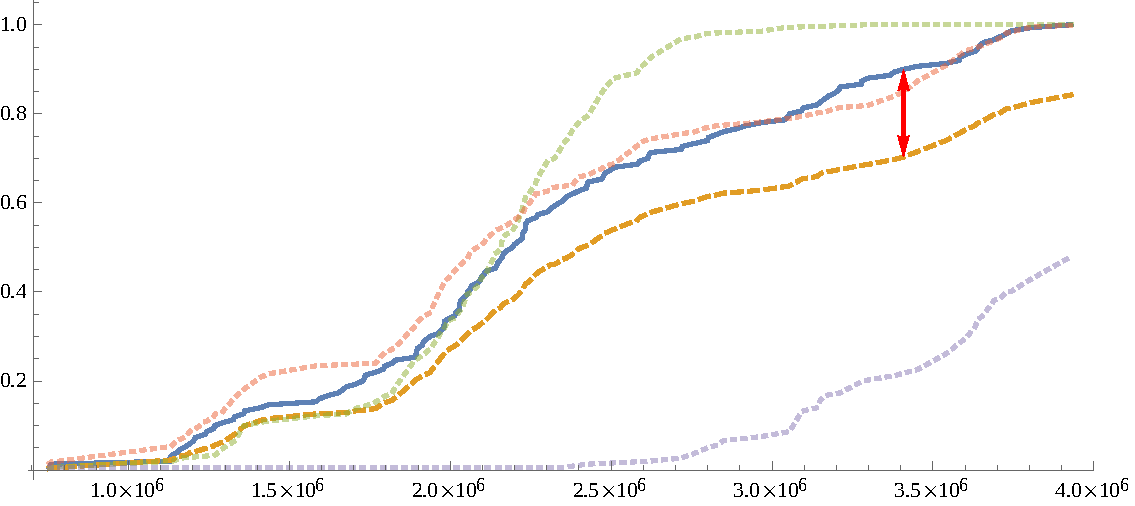
\includegraphics[width=0.75\textwidth,]{Figures/plot-delaunay-example-prediction.pdf}};
    \node[below=of img, node distance=1cm, yshift=1cm] {I/O Throughput};
    \node[left=of img, node distance=0cm, rotate=90, anchor=center,yshift=-0.7cm] {CDF Value};
  \end{tikzpicture}
  \vspace{-0.3cm}
  \caption{In this HPC I/O example, the general methodology for predicting a CDF and evaluating error can be seen. The Delaunay method chose three source distributions (dotted lines) and assigned weights \{.3, .4, .3\} (top to bottom at arrow). The weighted sum of the three known CDFs produces the predicted CDF (dashed line). The KS Statistic (arrow) computed between the true CDF (solid line) and predicted CDF (dashed line) is 0.2 for this example. The KS test null hypothesis is rejected at $p$-value 0.01, however it is not rejected at $p$-value 0.001.
  \vspace{-.1cm}}
  \label{fig:prediction-example}
\end{figure}

When the range of an approximation is the real numbers, error is reported with summary statistics including: min absolute error, max absolute error, and absolute error quartiles. When the range of an approximation is the space of cumulative distribution functions, the Kolmogorov-Smirnov statistic (max-norm difference between the functions) is used.

A hurdle when modeling function-valued outputs such as cumulative distribution functions (CDFs) or probability density functions (PDFs) is that certain properties must be maintained. It is necessary that a PDF $f: \mathbb{R} \rightarrow \mathbb{R}$ have the properties $f(x) \geq 0$ and $\int_{-\infty}^{\infty}f(x)dx = 1$. However, for a CDF $F: \mathbb{R} \rightarrow \mathbb{R}$ the properties are $F(x) \in [0,1]$ and $F(x)$ is absolutely continuous and nondecreasing. This work utilizes the fact that a convex combination of CDFs (or PDFs) results in a valid CDF. Given $G(x) = \sum_{i}w_i F_i(x)$, $\sum_{i} w_i = 1$, $w_i \geq 0$, and each $F_i$ is a valid CDF, $G$ must also be a valid CDF. A demonstration of how this is applied can be seen in Figure \ref{fig:prediction-example}.

The performance of approximation techniques that predict probability functions can be analyzed through a variety of summary statistics. This work uses the max absolute difference, also known as the Kolmogorov-Smirnov (KS) statistic \cite{lilliefors1967kolmogorov} for its compatibility with the KS test.

The two-sample KS test is a useful nonparametric test for comparing two CDFs while only assuming stationarity, finite mean, and finite variance. The null hypothesis (that two CDFs come from the same underlying distribution) is rejected at level $p \in [0,1]$ when
$$ KS > \sqrt{-\frac{1}{2}\ln\biggl(\frac{p}{2}\biggr)} \sqrt{\frac{1}{n_1} + \frac{1}{n_2}}, $$
with distribution sample sizes $n_1,n_2 \in \mathcal{N}$. For all applications of the KS test presented in this work $n_1 = n_2$. An example of the round-trip prediction methodology from known and predicted distributions to the calculation of error can be seen in Figure \ref{fig:prediction-example}.

\section{Theoretical Error Bound}
\label{sec:theory}

This section presents the theoretical results bounding the error of Delaunay interpolation. The error analysis relies on the Delaunay interpolation for two reasons: (1) second order results can be obtained utilizing a Lipschitz constant on the gradient of a function, rather than standard Lipschitz bounds and (2) multiple other interpolants analyzed compute predictions as convex combinations of observed function values, which may allow for straight forward extensions of this error bound.

\begin{plainlemma}
  \label{lemma:1}
  Let $S \subset \mathbb{R}^d$ be open and convex, $f: \mathbb{R}^d \rightarrow \mathbb{R}$, and $\nabla f \in Lip_{(\gamma,\|\cdot\|_2)}(S)$, the set of $\gamma$-Lipschitz continuous functions in the $2$-norm. Then for all $x,y \in S$
  $$\big|f(y) - f(x) - \langle \nabla f(x), y - x \rangle \big| \leq \frac{\gamma \|y - x\|_2^2}{2}.$$
\end{plainlemma}

\begin{proofdot}
  Consider the function $g(t) = f \big((1-t) x + t y \big)$, $0 \leq t \leq 1$, whose derivative $g'(t) = \big\langle \nabla f \big((1-t) x + t y \big), y - x \big\rangle$ is the directional derivative of $f$ in the direction $(y - x).$
  \begin{align*}
    \big|f(y) - f(x) - \langle \nabla f(x), y - x \rangle \big|
       &= \big|g(1) - g(0) - g'(0) \big| & \\
       &= \bigg| \int_0^1 g'(t) - g'(0)\ dt \bigg| \\
       &\leq \int_0^1 \big|g'(t) - g'(0)\big|\ dt \\
       &= \int_0^1 \bigg| \big \langle \nabla f\big((1-t)x + ty\big) - \nabla f(x), y - x \big \rangle \bigg|\ dt \\
       &\leq \int_0^1 \big \| \nabla f\big((1-t)x + ty\big) - \nabla f(x) \big \|_2\ \| y - x \|_2\ dt \\
       &\leq \int_0^1 \big ( \gamma\ \|y-x\|_2 \big) \ \big( \|y-x\|_2 \big) t\ dt \\
       &= \frac{\gamma \|y - x\|_2^2}{2}.
  \end{align*}
  \qed
\end{proofdot}

\begin{plainlemma}
  \label{lemma:2}
  Let $x, y, v_i \in \mathbb{R}^d$, $c_i \in \mathbb{R}$, and $|\langle y - x, v_i \rangle| \leq c_i$ for $i = 1$, $\ldots$, $d.$ If $M = (v_1$, $\ldots$, $v_d)$ is nonsingular, then
  $$\|y - x\|_2^2 \leq \frac{1}{\sigma_d^2} \sum_{i=1}^d c_i^2,$$
  where $\sigma_d$ is the smallest singular value of $M.$
\end{plainlemma}

\begin{proofdot}
  Using the facts that $M$ and $M^t$ have the same singular values, and $\|M^tw\|_2 \geq \sigma_d \|w\|_2$, gives
  \begin{align*}
    \|y - x\|_2^2 &\leq \frac{\|M^t (y - x)\|_2^2}{\sigma_d^2} \\
                  &=    \frac{1}{\sigma_d^2} \sum_{i=1}^d \langle y - x, v_i \rangle^2 \\
                  &\leq \frac{1}{\sigma_d^2} \sum_{i=1}^d c_i^2.
  \end{align*}
  \qed
\end{proofdot}

\begin{plainlemma}
  \label{lemma:3}
  Given $f$, $\gamma$, $S$ as in {\it Lemma \ref{lemma:1}}, let $X = \{x_0$, $x_1$, $\ldots$, $x_d\}$ $\subset S$ be the vertices of a $d$-simplex, and let $\hat f(x) = \langle c, x - x_0 \rangle + f(x_0)$, $c \in \mathbb{R}^d$ be the linear function interpolating $f$ on $X.$ Let $\sigma_d$ be the smallest singular value of the matrix $M = (x_1 - x_0$, $\ldots$, $x_d - x_0)$, and $k = \max\limits_{1\ \leq\ j\ \leq\ d} \|x_j - x_0\|_2.$ Then
  $$\big\|\nabla f(x_0) - c\big\|_2 \leq \sqrt{d} \frac{\gamma k^2}{\sigma_d}.$$
\end{plainlemma}

\begin{proofdot}
  Consider $f(x) - \hat f(x)$ along the line segment $z(t) = (1-t)x_0 + t x_j$, $0 \leq t \leq 1.$ By Rolle's Theorem, for some $0 < \hat t < 1$, $\big\langle \nabla f\big(z(\ \hat t\ )\big) - c, x_j - x_0 \big\rangle = 0.$ Now
  \begin{align*}
    \big| \big< \nabla f(x_0) - c, x_j - x_0 \big \rangle \big|
        &= \big| \big< \nabla f(x_0) - \nabla f\big(z(\ \hat t\ )\big) + \nabla f\big(z(\ \hat t\ )\big) - c, x_j - x_0 \big \rangle \big| \\
	&= \big| \big\langle \nabla f(x_0) - \nabla f \big(z(\ \hat t\ )\big), x_j - x_0 \big \rangle \big| \\
	&\leq \big \| \nabla f(x_0) - \nabla f\big(z(\ \hat t\ )\big) \big \|_2 \|x_j - x_0\|_2 \\
	&\leq \gamma \|x_0 - z(\ \hat t\ )\|_2\ \|x_j - x_0\|_2 \\
	&\leq \gamma \|x_j - x_0\|_2^2 \leq \gamma k^2, \\
  \end{align*}
  for all $1 \leq j \leq d.$ Using {\it Lemma \ref{lemma:2}},
  $$\big \| \nabla f(x_i) - c \big \|_2^2 \leq \frac{d}{\sigma_d^2} \big( \gamma k^2\big)^2 \implies \big \| \nabla f(x_i) - c \big \|_2 \leq \sqrt{d} \frac{\gamma k^2}{\sigma_d}.$$
  \qed
\end{proofdot}

\begin{onetheorem}
  Under the assumptions of {\it Lemma \ref{lemma:1}} and {\it Lemma \ref{lemma:3}}, for $z \in S$,
  $$ \big|f(z) - \hat f(z)\big| \leq \frac{\gamma \|z - x_0\|_2^2}{2} + \sqrt{d} \frac{\gamma k^2}{\sigma_d} \|z - x_0\|_2.$$
\end{onetheorem}

\begin{proofdot}
  Let $v = \nabla f(x_0) - c$, where $\|v\|_2 \leq \sqrt{d} \gamma k^2 / \sigma_d$ by {\it Lemma \ref{lemma:3}}. Now
  \begin{align*}
    \big|f(z) - \hat f(z)\big|
       &= \big|f(z) - f(x_0) - \langle c, z - x_0 \rangle \big| \\ 
       &= \big|f(z) - f(x_0) - \langle \nabla f(x_0) - v, z - x_0 \rangle \big| \\
       &= \big|f(z) - f(x_0) - \langle \nabla f(x_0) , z - x_0 \rangle + \langle v , z - x_0 \rangle \big| \\
       &\leq \big|f(z) - f(x_0) - \langle \nabla f(x_0) , z - x_0 \rangle \big| + \big| \langle v , z - x_0 \rangle \big| \\
       &\leq \big|f(z) - f(x_0) - \langle \nabla f(x_0) , z - x_0 \rangle \big| + \|v\|_2 \|z - x_0\|_2 \\
       &\leq \big|f(z) - f(x_0) - \langle \nabla f(x_0), z - x_0 \rangle \big| + \textstyle{\frac{\gamma k^2 \sqrt{d}}{\sigma_d}} \|z - x_0\|_2 \\
       &\leq \frac{\gamma \|z - x_0\|_2^2}{2} + \sqrt{d}\frac{\gamma k^2}{\sigma_d} \|z - x_0\|_2,
  \end{align*}
  where the last inequality follows from {\it Lemma \ref{lemma:1}}.
  %
  \qed
\end{proofdot}


In summary, the approximation error of a Delaunay interpolant tends quadratically towards zero when approaching observed data only when the diameter of the interpolating simplex is also reduced at a proportional rate. Without the incorporation of additional observations, only linear convergence to the true function is be achieved. Notice that the approximation error is largely determined by the spacing of observed data. Predictions made by simplices whose vertices are not well-spaced (i.e. have large diameter, or are nearly contained in a hyperplane) have higher error. In light of this error bound, an empirical evaluation of presented algorithms follows.

%% ===================================================================
\section{Data and Empirical Analysis}
\label{sec:data}

The theoretical results constructed in Section \ref{sec:theory} for Delaunay interpolation are promising, however they are difficult to interpret in context with the other approximation algorithms that do not have similar known uniform error bounds. For that reason, this paper utilizes five different data sets of varying dimension and application to construct approximations and compare the accuracy of different techniques.

In the following five subsections the sources and targets of each test data set are described, as well as challenges and limitations related to approximating these data. The distribution of response values being modeled is presented followed by the distribution of approximation errors for each algorithm.

Before approximations are constructed, all five data sets are rescaled such that the domain of approximation is the unit hypercube. The range of the first four data sets is the real numbers, while the range of the fifth data set is the space of cumulative distribution functions. All approximation techniques are applied to the first four data sets, while only those interpolants whose approximations are convex combinations of observed data are applied to the final data set.

All approximations are constructed using $10$-fold cross validation as described in \cite{kohavi1995study}. This approach requires the division of data randomly into $10$ partitions (the same partitions are used by each algorithm). An algorithm is then evaluated by constructing an approximation over each set of $9$ partitions, predicting the values of the final partition. As a result, each observed data point is used in the construction of $9$ different approximations and is approximated exactly once. The $k$-fold cross validation method is data-efficient and provides an unbiased estimate of the expected prediction error \cite{kohavi1995study}, however it should be noted that neither this method nor others can provide a universally unbiased estimator for the variance of prediction error \cite{bengio2004no}.

In addition to the figures displaying approximation results for each data set, tables of accompanying numerical results are located in the Appendix. All of the test data sets capture underlying functions that are almost certainly stochastic. As described in Section \ref{sec:introduction}, regression techniques appear most appropriate for these problems. However, in high dimension data grows exponentially more sparse. Given sparse data, regressors tend towards interpolation.

%% -------------------------------------------------------------------
\subsection{Forest Fire ($n = 504, d = 12$)}

\begin{figure}
  \centering
  \begin{tikzpicture}
    \node (img)  {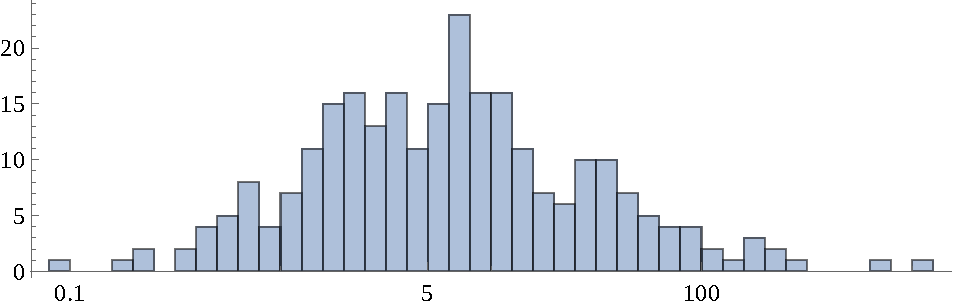
\includegraphics[width=0.75\textwidth,]{Figures/raw-histogram-forest-fire.pdf}};
    \node[below=of img, node distance=1cm, yshift=1cm] {Forest First Area Burned};
    \node[left=of img, node distance=0cm, rotate=90, anchor=center,yshift=-0.7cm] {Count};
  \end{tikzpicture}
  \caption{Above is a histogram of forest fire area burned under recorded weather conditions. The data is presented on a natural log scale because most values are small with exponentially fewer fires on record that burn large areas.}
  \label{fig:hist-forest-fire}
\end{figure}

\begin{figure}
  \centering
  \begin{tikzpicture}
    \node (img)  {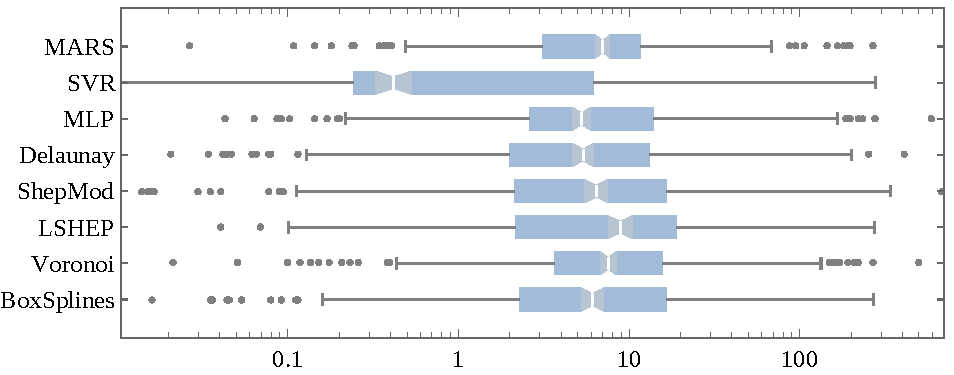
\includegraphics[width=0.8\textwidth,]{Figures/error-box-forest-fire.pdf}};
    \node[below=of img, node distance=1cm, yshift=1cm] {Area Burned Error};
  \end{tikzpicture}
  \caption{All models are applied to approximate the amount of area that would be burned given environment conditions. The data is broken up into $10$ partitions and each set of $9$ partitions is used to construct a model that approximates the remaining partition. This results in exactly one prediction from each algorithm for each data point. These boxes depict the median (middle bar), median $95\%$ confidence interval (cones), quartiles (box edges), fences at $3/2$ interquartile range (whiskers), and outliers (dots) of absolute prediction error for each model. Similar to figure \ref{fig:hist-forest-fire}, the errors are presented on a natural log scale. The complementing numerical data to this figure is provided in table \ref{table:error-forest-fire} in the Appendix.}
  \label{fig:error-forest-fire}
\end{figure}


The forest fire data set \cite{cortez2007data} describes the area of Montesinho park burned over months of the year along with environmental conditions. The twelve dimensions being used to model burn area are the $x$ and $y$ spatial coordinates of burns in the park, month of year (mapped to a 2D circle), the FFMC, DMC, DC, and ISI indices (see source for details), the temperature, relative humidity, wind speed, and outdoor rain. The original analysis of this data set demonstrated it to be difficult to model, likely due to the skew in response values.

As suggested by figure \ref{fig:error-forest-fire}, the SVR has the lowest absolute prediction errors for 80\% of the data, with ShepMod and BoxSpline being the nearest overall competitors. The effectiveness of SVR on this data suggests the underlying function can be defined by relatively few parameters, as well as the importance of capturing the low-burn-area data points.
%% -------------------------------------------------------------------



%% -------------------------------------------------------------------
\subsection{Parkinson's Telemonitoring ($n = 5875, d = 19$)}

\begin{figure}
  \centering
  \begin{tikzpicture}
    \node (img)  {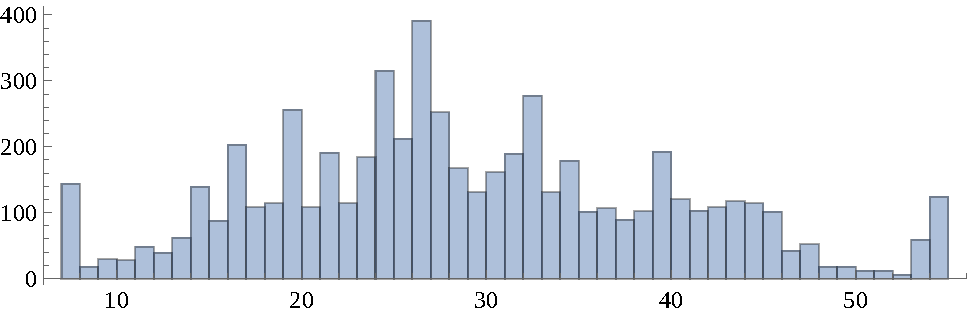
\includegraphics[width=0.75\textwidth,]{Figures/raw-histogram-parkinsons.pdf}};
    \node[below=of img, node distance=1cm, yshift=1cm] {Parkinson's Total UPDRS Score};
    \node[left=of img, node distance=0cm, rotate=90, anchor=center,yshift=-0.7cm] {Count};
  \end{tikzpicture}
  \caption{Above is a histogram of the Parkinson's patient total UPDRS clinical scores that will be approximated by each algorithm.}
  \label{fig:hist-parkinsons}
\end{figure}

\begin{figure}
  \centering
  \begin{tikzpicture}
    \node (img)  {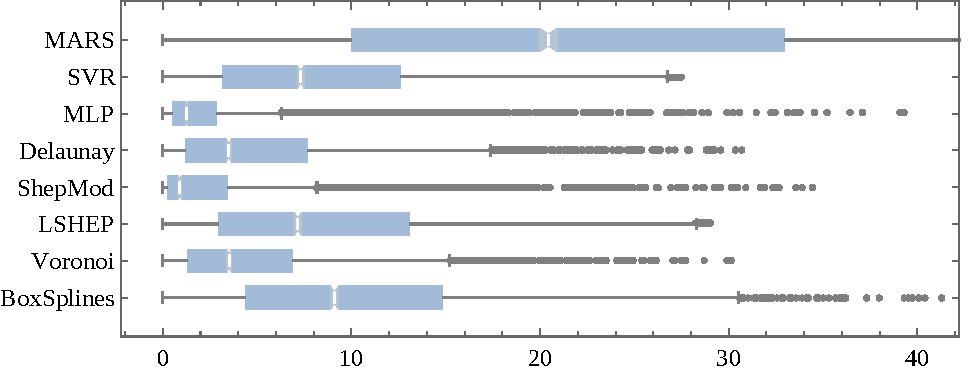
\includegraphics[width=0.8\textwidth,]{Figures/error-box-parkinsons.pdf}};
    \node[below=of img, node distance=1cm, yshift=1cm] {Total UPDRS Score Error};
  \end{tikzpicture}
  \caption{All models are applied to approximate the total UPDRS score given audio features from patients' home life. The data is broken up into $10$ partitions and each set of $9$ partitions is used to construct a model that approximates the remaining partition. This results in exactly one prediction from each algorithm for each data point. These boxes depict the median (middle bar), median $95\%$ confidence interval (cones), quartiles (box edges), fences at $3/2$ interquartile range (whiskers), and outliers (dots) of absolute prediction error for each model. The complementing numerical data to this is provided in table \ref{table:error-parkinsons} in the Appendix.}
  \label{fig:error-parkinsons}
\end{figure}

The second data set for evaluation \cite{tsanas2010accurate} is derived from a speech monitoring study with the intent to automatically estimate Parkinson's disease symptom development in Parkinson's patients. The function to be approximated is a time-consuming clinical evaluation measure referred to as the UPDRS score. The total UPDRS score given by a clinical evaluation is estimated through 16 real numbers generated from biomedical voice measures of in-home sound recordings.

Figure \ref{fig:error-parkinsons} shows the ShepMod algorithm has the lowest minimum, first quartile, and median of absolute errors for this problem, while providing the best prediction 66\% of the time. The MLP has the lowest third quartile and provides the best prediction for 32\% of approximations. The dominance of ShepMod may be in part to regular-interval total UPDRS scores provided by clinicians, favoring a nearest-neighbor strategy of prediction.
%% -------------------------------------------------------------------



%% -------------------------------------------------------------------
\subsection{Australian Daily Rainfall Volume ($n = 2609, d = 23$)}

\begin{figure}
  \centering
  \begin{tikzpicture}
    \node (img)  {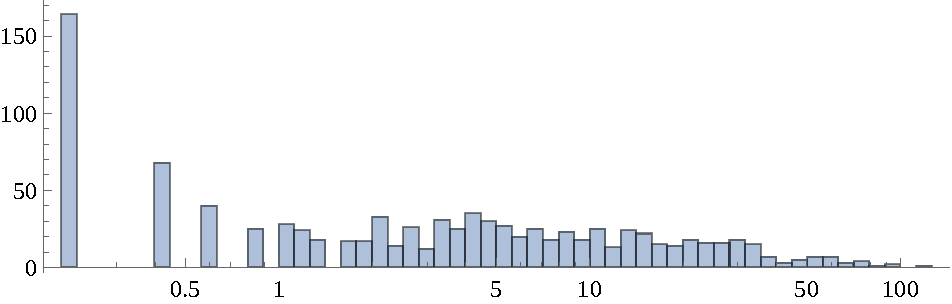
\includegraphics[width=0.75\textwidth,]{Figures/raw-histogram-weather.pdf}};
    \node[below=of img, node distance=1cm, yshift=1cm] {Daily Rainfall in Sydney};
    \node[left=of img, node distance=0cm, rotate=90, anchor=center,yshift=-0.7cm] {Count};
  \end{tikzpicture}
  \caption{Above is a histogram of daily rainfall in Sydney, Australia. The data is presented on a natural log scale because the frequency of larger amounts of rainfall is significantly less. There is a peak in occurrence of the value $0$, which has a notable effect on the resulting model performance.}
  \label{fig:hist-weather}
\end{figure}

\begin{figure}
  \centering
  \begin{tikzpicture}
    \node (img)  {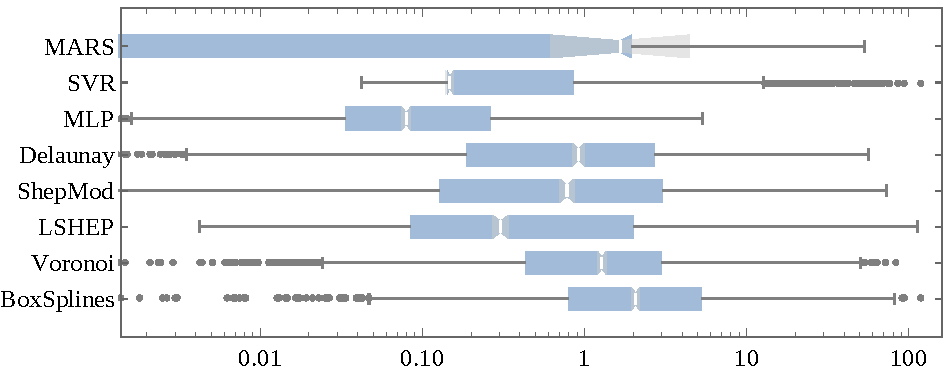
\includegraphics[width=0.8\textwidth,]{Figures/error-box-weather.pdf}};
    \node[below=of img, node distance=1cm, yshift=1cm] {Sydney Rainfall Tomorrow Error};
  \end{tikzpicture}
  \caption{All models are applied to approximate the amount of rainfall expected on the next calendar day given various sources of local meteorological data. The data is broken up into $10$ partitions and each set of $9$ partitions is used to construct models that approximates the remaining partition. This results in exactly one prediction from each algorithm for each data point. These boxes depict the median (middle bar), median $95\%$ confidence interval (cones), quartiles (box edges), fences at $3/2$ interquartile range (whiskers), and outliers (dots) of absolute prediction error for each model. The errors are presented on a natural log scale, mimicking the presentation in figure \ref{fig:hist-weather}. The complementing numerical data to this figure is provided in table \ref{table:error-weather} in the Appendix.}
  \label{fig:error-weather}
\end{figure}

The third data regarding the total daily rainfall in Sydney, Australia \cite{williams2009rattle} provides a slightly higher dimension challenge for the interpolants and regressors. This data is composed of many meteorological readings from the region on a day including: min and max temperatures, sunshine, wind speed directions (converted to coordinates on circle), wind speeds, and humidities throughout the day, day of the year (converted to coordinates on circle), and the model must predict the amount of rainfall tomorrow.

While figure \ref{fig:hist-weather} makes MARS look far better than other techniques, it only provides the best prediction for 11\% of points. The MLP has the lowest absolute error for 56\% of points and LSHEP is best for 28\%. MARS likely achieves such a low first quartile due to the high occurrence of the value 0 in the data.
%% -------------------------------------------------------------------



%% -------------------------------------------------------------------
\subsection{Credit Card Transaction Amount ($n = 5562, d = 28$)}

\begin{figure}
  \centering
  \begin{tikzpicture}
    \node (img)  {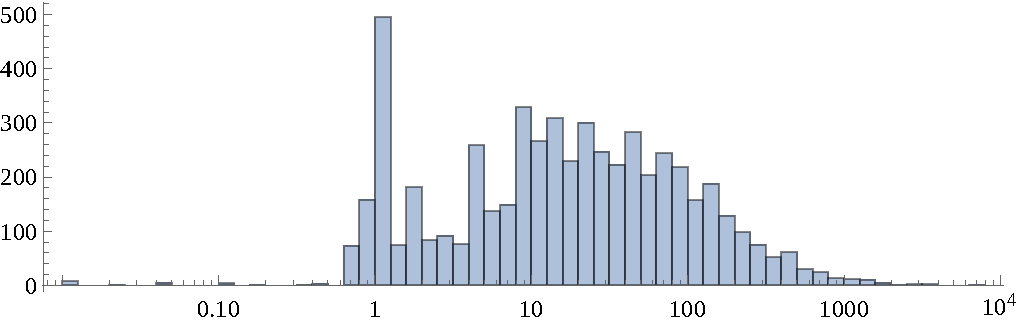
\includegraphics[width=0.75\textwidth,]{Figures/raw-histogram-credit-card.pdf}};
    \node[below=of img, node distance=1cm, yshift=1cm] {Credit Card Transaction Amount};
    \node[left=of img, node distance=0cm, rotate=90, anchor=center,yshift=-0.7cm] {Count};
  \end{tikzpicture}
  \caption{Above is a histogram of credit card transaction amounts. The data is presented on a natural log scale. The data contains a notable frequency peak around $\$1$ transactions. Fewer large purchases are made, but some large purchases are in excess of five orders of magnitude greater than the smallest purchases.}
  \label{fig:hist-credit-card}
\end{figure}

\begin{figure}
  \centering
  \begin{tikzpicture}
    \node (img)  {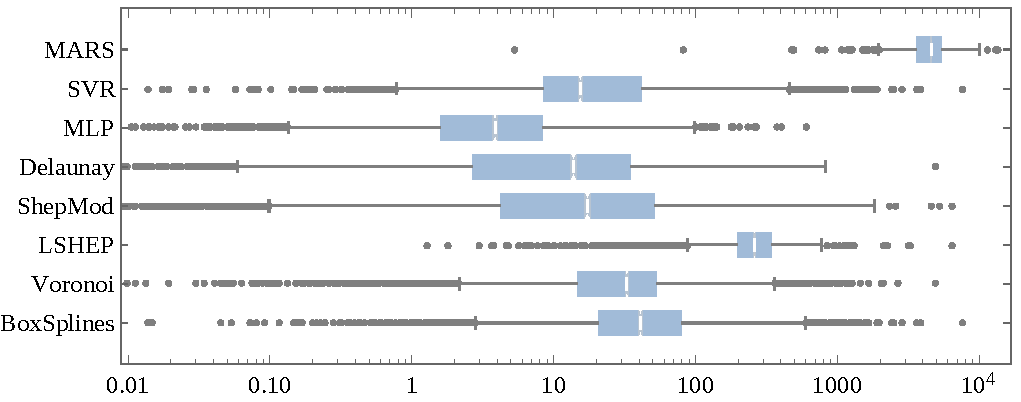
\includegraphics[width=0.8\textwidth,]{Figures/error-box-credit-card.pdf}};
    \node[below=of img, node distance=1cm, yshift=1cm] {Transaction Amount Error};
  \end{tikzpicture}
  \caption{All models are applied to approximate the expected transaction amount given transformed (and obfuscated) vendor and customer-descriptive features. The data is broken up into $10$ partitions and each set of $9$ partitions is used to construct a model that approximates the remaining partition. This results in exactly one prediction from each algorithm for each data point. These boxes depict the median (middle bar), median $95\%$ confidence interval (cones), quartiles (box edges), fences at $3/2$ interquartile range (whiskers), and outliers (dots) of absolute prediction error for each model. The absolute errors in transaction amount predictions are presented on a natural log scale, just as in figure \ref{fig:hist-credit-card}. The complementing numerical data to this figure is provided in table \ref{table:error-credit-card} in the Appendix.}
  \label{fig:error-credit-card}
\end{figure}

The fourth test data set, and the final with a real-valued range, is a collection of credit card transactions \cite{pozzolo2015calibrating}. The provided data carries no direct real-world meaning, it is the output of a principle component analysis on the original hidden source data. This obfuscation is done to protect the information of the credit card users. This data has the largest dimension of all considered, at 28. A model over this data predicts the transaction amount given the vector of principle component information.

As can be seen in figure \ref{fig:error-credit-card}, the MLP outperforms all other algorithms at the first, second, third, and fourth quartiles. The MLP produces the lowest absolute error prediction for 80\% of transactions, Delaunay bests the remaining 20\%. It is likely that with less data, Delaunay would be the best performer.
%% -------------------------------------------------------------------


%% -------------------------------------------------------------------
\subsection{High Performance Computing I/O ($n = 3016, d = 4$)}

\begin{figure}
  \centering
  \begin{tikzpicture}
    \node (img)  {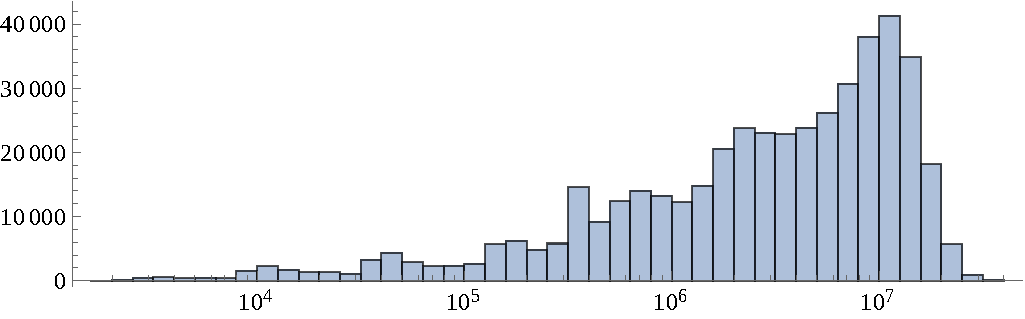
\includegraphics[width=0.75\textwidth,]{Figures/raw-histogram-throughput.pdf}};
    \node[below=of img, node distance=1cm, yshift=1cm] {I/O Read Throughtput};
    \node[left=of img, node distance=0cm, rotate=90, anchor=center,yshift=-0.7cm] {Count};
  \end{tikzpicture}
  \caption{Histogram of the raw throughput values recorded during all IOzone tests across all system configurations. The distribution is skewed right, with few tests having significantly higher throughput than most others. The data is presented on a natural log scale, however the resulting left-skew reveals the data is not precisely distributed according to an exponential.}
  \label{fig:hist-throughput}
\end{figure}

\begin{figure}
  \centering
  \begin{tikzpicture}
    \node (img)  {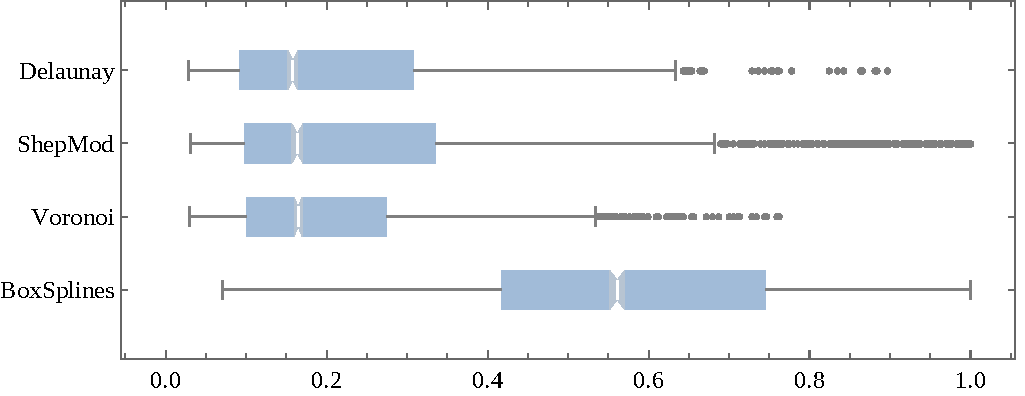
\includegraphics[width=0.8\textwidth,]{Figures/error-box-throughput.pdf}};
    \node[below=of img, node distance=1cm, yshift=1cm] {Read Throughtput KS Statistic};
  \end{tikzpicture}
  \caption{Above, the models directly capable of predicting distributions are applied to predicting the expected CDF of I/O throughput at a previously unseen system configuration. The KS statistic between the observed distribution at each system configuration and the predicted distribution is recorded and presented above. Note that the above plot is \textit{not} log-scaled like the histogram. The complimentary numerical data for this figure is provided in Appendix table \ref{table:error-throughput}.}
  \label{fig:error-throughput}
\end{figure}

The final of five data sets is four-dimensional and is produced by executing the IOzone benchmark from \cite{iozone} on a homogeneous cluster of computers. The system performance data was collected by executing IOzone 150 times for each of a select set of system configurations. A single IOzone execution reports the max I/O file-read throughput seen. The 150 executions for each system configuration are converted
to their empirical distribution function point, which are fit with a piecewise cubic Hermite interpolating polynomial \cite{fritsch1980monotone} to approximate the CDF. These CDFs are capable of being approximated by all interpolants except LSHEP. The four dimensions being modeled to predict throughput mean are file size, record size, thread count, and CPU frequency.

Delaunay achieves the lowest KS statistic for 62\% of approximations, while Voronoi is best for the remaining 38\%. Figure \ref{fig:error-throughput} shows that while Delaunay may have more best predictions, the behavior of Voronoi may be preferable.
%% -------------------------------------------------------------------


%% -------------------------------------------------------------------
\begin{figure}
  \centering
  \begin{tikzpicture}
    \node (img)  {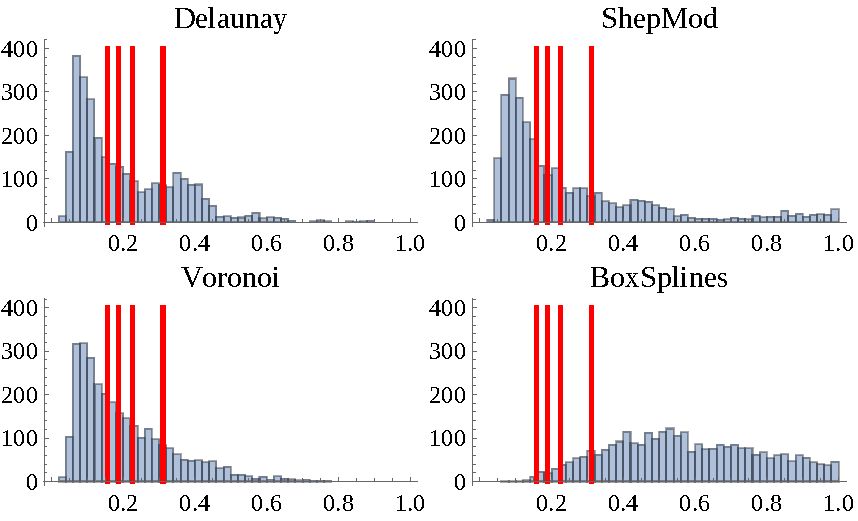
\includegraphics[width=0.8\textwidth]{Figures/plot-throughput-ks.pdf}};
    \node[below=of img, node distance=1cm, yshift=1cm] {KS Statistic for Predicted vs. Actual};
    \node[left=of img, node distance=0cm, rotate=90, anchor=center,yshift=-0.7cm] {Count of KS Statistic};
  \end{tikzpicture}
  \caption{Histograms of the prediction error for each interpolant that produces predictions as convex combinations of observed data. The data is broken up into $10$ partitions and each set of $9$ partitions is used to construct a model that approximates the remaining partition. This results in exactly one prediction from each algorithm for each data point. The distributions show the KS statistics for the predicted throughput distribution versus the actual throughput distribution. The four vertical red lines represent commonly used $p$-values \{0.05, 0.01, 0.001, 1.0e-6\} respectively. All predictions to the right of a red line represent CDF predictions that are significantly different (by respective $p$-value) from the actual distribution according to the KS test. The numerical counterpart to this figure is presented in table \ref{table:null-hypothesis-results}.}
  \label{fig:throughput-prediction}
\end{figure}

\begin{table}
  \renewcommand{\arraystretch}{1.3}
  \centering
  \begin{tabular}{c|c|c|c|c}
     & $p$ = .05 & $p$ = .01 & $p$ = .001 & $p$ = 1.0e-6\\
    \hline
    Delaunay & $\mathbf{50.3}\%$ & $\mathit{43.5}\%$ & $\mathit{36.2}\%$ & $\mathit{24.7}\%$\\
    ShepMod & $\mathit{51.4}\%$ & $44.8\%$ & $38.1\%$ & $27.7\%$\\
    Voronoi & $52.6\%$ & $\mathbf{43.4}\%$ & $\mathbf{34.4}\%$ & $\mathbf{19.1}\%$\\
    BoxMesh & $99.5\%$ & $98.5\%$ & $96.6\%$ & $89.5\%$\\
  \end{tabular}
  \caption{This is the numerical counterpart to the histogram data presented in figure \ref{fig:throughput-prediction}. The columns display the percent of null hypothesis rejections by the KS-test when provided different selections of $p$-values for each algorithm. The algorithm with the lowest rejection rate at each $p$ is boldface, while the second lowest is italicized.}
  \label{table:null-hypothesis-results}
\end{table}


%% ===================================================================

Figure \ref{fig:throughput-prediction} expands on the KS statistic results presented in figure \ref{fig:error-throughput}. Agglomerate errors for each algorithm resemble a Gamma distribution. The percentages of significant prediction errors with varying $p$-values are on display in Table \ref{table:null-hypothesis-results}. When considering the $p=0.001$ results for each technique, a little over one third of the predicted CDFs are significantly different from the measured (and presumed) correct CDFs. However, it should be noted that with 150 samples, the error of an empirical distribution function (EDF) can reasonably be upwards of $.1$, which serves as a rough estimate for the lower limit of achievable error. Globally, only a third of Voronoi predictions fail to capture \textit{all} of the characteristics of the CDFs at new system configurations.

\section{Discussion}
\label{sec:discussion}

                                                                      
\begin{table}
  \centering
  \begin{tabular}{c|c|c|c}
    \hline
    Algorithm & Avg. \% Best & Avg. Fit Time & Avg. App. Time (1)\\
    \hline
    MARS & $4.6\%$ & $22.3$s & $1.37 \times 10^{-3}$s\\
    SVR & $\mathit{21.1}\%$ & $0.503$s & $\mathit{1.37 \times 10^{-4}}$s\\
    MLP & $\mathbf{42.1}\%$ & $210.0$s & $1.02 \times 10^{-3}$s\\
    Delaunay & $6.0\%$ & $\mathbf{1.43 \times 10^{-4}}$s & $3.03$s\\
    ShepMod & $18.4\%$ & $0.711$s & $1.49 \times 10^{-4}$s\\
    LSHEP & $8.4\%$ & $1.69$s & $\mathbf{1.16 \times 10^{-4}}$s\\
    Voronoi & $0.5\%$ & $\mathit{0.127}$s & $0.0375$s\\
    BoxSplines & $0.2\%$ & $0.816$s & $5.26 \times 10^{-4}$s\\
    \hline
  \end{tabular}
  \caption{This data is the average of Appendix tables \ref{table:error-forest-fire}, \ref{table:error-parkinsons}, \ref{table:error-weather}, \ref{table:error-credit-card}, and provides a gross summary of overall results. The columns display (weighted equally by data set, \textit{not} points) the average frequency with which any algorithm provided the lowest absolute error approximation, the average time-to-fit, and the average time required to approximated one point. Interpolants provide the lowest error approximation one third of the time across all data, while regressors occupy the other two thirds. This result is obtained without any customized tuning or preprocessing to maximize the performance of any given algorithm. In practice, tuning and preprocessing may have large effects on approximation performance.}
  \label{table:avg-performance}
\end{table}

Table \ref{table:avg-performance} summarizes results across the four test data sets with real-valued ranges. The interpolants discussed in this paper produce the \textit{best} approximations roughly one third of the time, and produce competitive approximations for almost all data sets. These test problems are almost certainly \textit{stochastic} in nature, but the high dimension yields to greater sparsity and makes interpolation a competitive approximation technique.

The major advantages to interpolation lie in the near absence of \textit{fit} time. Delaunay has no preparations required, LSHEP and ShepMod require pairwise distance calculations to determine the radii of influence for points in each model. At least hundreds, and sometimes hundreds of thousands of predictions can be made by the interpolants before the most widely used regressor (the MLP) finishes fitting these relatively small data sets. However, the computational complexities of all interpolants presented are greater than linear in either dimension or number of points, meaning large enough data (in dimension and number of observations) would cause interpolation to be slower.

The theoretical results presented in Section \ref{sec:theory} directly apply to Delaunay interpolation, however the performance of Delaunay does not appear significantly better than other algorithms on these data sets. This observation may be due to the stochastic nature of the data, but it also speaks to the alignment of the geometry of the underlying functions with the approximations generated by the different interpolation methods. The strong performance of other interpolants suggests that theoretical results similar to those presented in this work can be achieved for the other interpolants under reasonable assumptions.

Finally, most of the interpolants presented in this work benefit from the ability to model any function over a real vector space with a range that is closed under convex combinations. The results of the distribution prediction case study indicate that interpolants can effectively predict CDFs. The error analysis for that work relies on the KS statistic, which captures the worst part of any prediction and hence provides a conservatively large estimate of approximation error. The average absolute errors in the predicted CDFs are always lower than the KS statistics. However, the KS statistic was chosen because of the important statistical theory surrounding it as an error measure. Considering this circumstance, a nonnegligible volume of predictions provide impressively low levels of error in that final case study.


\section{Conclusion}
\label{sec:conclusion}

This work presents new theoretical results for interpolation in arbitrary dimension with simplicial approximations. Coinciding with the theoretical results, an empirical evaluation across real-world problems demonstrates that interpolants produce competitively accurate models of multivariate phenomenon when compared with common regressors for sparse, moderately high dimensional problems.

The various interpolants discussed in this paper have been demonstrated to effectively approximate multivariate phenomena up to $30$ dimensions. The underlying constructions are theoretically straightforward, yet powerful and flexible. Most of the interpolants' computational complexities make them particularly suitable for applications in even higher dimension, where the major benefits are seen when only a small number of approximations are to be made from any given data ($\leq 1000$).

%\begin{acknowledgements}
%If you'd like to thank anyone, place your comments here
%and remove the percent signs.
%\end{acknowledgements}

%%====================================================================
%%====================================================================

\bibliographystyle{spmpsci}      % mathematics and physical sciences
\bibliography{paper}

\begin{appendix}

\section*{Appendix}

\begin{table}
  \centering
  \begin{tabular}{c|c|c|c|c|c}
    \hline
    Algorithm & Min & $25^{th}$ & $50^{th}$ & $75^{th}$ & Max\\
    \hline
    MARS & $0.00984$ & $3.11$ & $7.01$ & $\mathit{11.7}$ & $1090.0$\\
    SVR & $\mathit{0.00402}$ & $\mathbf{0.243}$ & $\mathbf{0.416}$ & $\mathbf{6.19}$ & $1090.0$\\
    MLP & $0.0426$ & $2.63$ & $\mathit{5.27}$ & $14.0$ & $1090.0$\\
    Delaunay & $\mathbf{0.00}$ & $1.98$ & $5.37$ & $13.1$ & $\mathit{1080.0}$\\
    ShepMod & $\mathbf{0.00}$ & $\mathit{1.93}$ & $6.27$ & $16.0$ & $1090.0$\\
    LSHEP & $0.0400$ & $2.17$ & $8.87$ & $19.1$ & $\mathbf{1070.0}$\\
    Voronoi & $0.00982$ & $3.65$ & $7.56$ & $15.6$ & $1090.0$\\
    BoxSpline & $\mathbf{0.00}$ & $2.27$ & $5.91$ & $16.4$ & $1090.0$\\
    \hline
  \end{tabular}
  \caption{This numerical data accompanies the visual provided in figure \ref{fig:error-forest-fire}. The columns of absolute error percentiles correspond to the minimum, first quartile, median, second quartile, and maximum absolute errors respectively. The minimum of each column is boldface, while the second lowest value is italicized. All values are rounded to three significant digits.}
  \label{table:error-forest-fire}
\end{table}

\begin{table}
  \centering
  \begin{tabular}{|c|c| c |c|c|c|}
    \cline{1-2}\cline{4-6}
    Algorithm & \% Best &  & Fit Time & App. Time (1) & Total App. Time\\
    \cline{1-2}\cline{4-6}
    MARS & $\mathit{7.7}\%$ &  & $29.1$s & $1.37 \times 10^{-3}$s & $0.0686$s\\
    SVR & $\mathbf{80.2}\%$ &  & $5.84 \times 10^{-3}$s & $\mathit{6.20 \times 10^{-5}}$s & $\mathit{3.10 \times 10^{-3}}$s\\
    MLP & $0.0\%$ &  & $32.8$s & $8.71 \times 10^{-4}$s & $0.0436$s\\
    Delaunay & $3.5\%$ &  & $\mathbf{2.49 \times 10^{-5}}$s & $0.0385$s & $1.93$s\\
    ShepMod & $3.7\%$ &  & $6.34 \times 10^{-3}$s & $6.44 \times 10^{-5}$s & $3.22 \times 10^{-3}$s\\
    LSHEP & $5.1\%$ &  & $0.0275$s & $\mathbf{4.63 \times 10^{-5}}$s & $\mathbf{2.31 \times 10^{-3}}$s\\
    Voronoi & $0.0\%$ &  & $\mathit{1.82 \times 10^{-4}}$s & $3.96 \times 10^{-4}$s & $0.0198$s\\
    BoxSpline & $0.4\%$ &  & $7.24 \times 10^{-3}$s & $9.78 \times 10^{-5}$s & $4.89 \times 10^{-3}$s\\
    \cline{1-2}\cline{4-6}
  \end{tabular}
  \caption{The left above shows how often each algorithm had the lowest absolute error approximating forest fire data. On the right columns are median fit time of 454 points, median time for one approximation, and median time approximating 50 points.}
  \label{table:best-forest-fire}
\end{table}


\begin{table}
  \centering
  \begin{tabular}{c|c|c|c|c|c}
    \hline
    Algorithm & Min & $25^{th}$ & $50^{th}$ & $75^{th}$ & Max\\
    \hline
    MARS & $0.00948$ & $9.98$ & $20.4$ & $32.9$ & $863.0$\\
    SVR & $0.00138$ & $3.17$ & $7.31$ & $12.6$ & $\mathbf{27.5}$\\
    MLP & $2.39 \times 10^{-5}$ & $\mathit{0.533}$ & $\mathit{1.25}$ & $\mathbf{2.84}$ & $39.3$\\
    Delaunay & $\mathit{3.72 \times 10^{-12}}$ & $1.20$ & $3.50$ & $7.67$ & $30.7$\\
    ShepMod & $\mathbf{0.00}$ & $\mathbf{0.255}$ & $\mathbf{0.908}$ & $\mathit{3.43}$ & $34.5$\\
    LSHEP & $0.00254$ & $2.93$ & $7.16$ & $13.1$ & $\mathit{29.0}$\\
    Voronoi & $\mathbf{0.00}$ & $1.29$ & $3.52$ & $6.87$ & $30.1$\\
    BoxSpline & $0.00287$ & $4.39$ & $9.10$ & $14.8$ & $41.3$\\
    \hline
  \end{tabular}
  \caption{This numerical data accompanies the visual provided in figure \ref{fig:error-parkinsons}. The columns of absolute error percentiles correspond to the minimum, first quartile, median, second quartile, and maximum absolute errors respectively. The minimum of each column is boldface, while the second lowest value is italicized. All values are rounded to three significant digits.}
  \label{table:error-parkinsons}
\end{table}

\begin{table}
  \centering
  \begin{tabular}{|c|c| c |c|c|c|}
    \cline{1-2}\cline{4-6}
    Algorithm & \% Best &  & Fit Time & App. Time (1) & Total App. Time\\
    \cline{1-2}\cline{4-6}
    MARS & $0.0\%$ &  & $37.9$s & $2.53 \times 10^{-3}$s & $1.48$s\\
    SVR & $0.1\%$ &  & $0.859$s & $\mathit{1.81 \times 10^{-4}}$s & $\mathit{0.106}$s\\
    MLP & $\mathit{32.0}\%$ &  & $348.0$s & $1.11 \times 10^{-3}$s & $0.653$s\\
    Delaunay & $0.0\%$ &  & $\mathbf{1.90 \times 10^{-4}}$s & $3.69$s & $2.17 \times 10^{3}$s\\
    ShepMod & $\mathbf{66.4}\%$ &  & $1.13$s & $1.82 \times 10^{-4}$s & $0.107$s\\
    LSHEP & $0.0\%$ &  & $2.39$s & $\mathbf{1.44 \times 10^{-4}}$s & $\mathbf{0.0845}$s\\
    Voronoi & $1.6\%$ &  & $\mathit{0.298}$s & $0.0274$s & $16.1$s\\
    BoxSpline & $0.0\%$ &  & $1.26$s & $6.43 \times 10^{-4}$s & $0.377$s\\
    \cline{1-2}\cline{4-6}
  \end{tabular}
  \caption{The left above shows how often each algorithm had the lowest absolute error approximating parkinsons data. On the right columns are median fit time of 5288 points, median time for one approximation, and median time approximating 587 points.}
  \label{table:best-parkinsons}
\end{table}


\begin{table}
  \centering
  \begin{tabular}{c|c|c|c|c|c}
    \hline
    Algorithm & Min & $25^{th}$ & $50^{th}$ & $75^{th}$ & Max\\
    \hline
    MARS & $\mathit{6.45 \times 10^{-15}}$ & $\mathbf{2.70 \times 10^{-14}}$ & $1.66$ & $1.96$ & $\mathit{53.3}$\\
    SVR & $0.0420$ & $0.143$ & $0.148$ & $\mathit{0.860}$ & $119.0$\\
    MLP & $6.89 \times 10^{-5}$ & $0.0337$ & $\mathbf{0.0795}$ & $\mathbf{0.264}$ & $\mathbf{5.31}$\\
    Delaunay & $\mathbf{0.00}$ & $0.187$ & $0.919$ & $2.72$ & $56.3$\\
    ShepMod & $\mathbf{0.00}$ & $0.0957$ & $0.685$ & $2.90$ & $73.2$\\
    LSHEP & $\mathbf{0.00}$ & $\mathit{0.0153}$ & $\mathit{0.106}$ & $1.17$ & $113.0$\\
    Voronoi & $\mathbf{0.00}$ & $0.430$ & $1.28$ & $2.94$ & $83.8$\\
    BoxSpline & $\mathbf{0.00}$ & $0.789$ & $2.06$ & $5.25$ & $119.0$\\
    \hline
  \end{tabular}
  \caption{This numerical data accompanies the visual provided in figure \ref{fig:error-weather}. The columns of absolute error percentiles correspond to the minimum, first quartile, median, second quartile, and maximum absolute errors respectively. The minimum value of each column is boldface, while the second lowest is italicized. All values are rounded to three significant digits.}
  \label{table:error-weather}
\end{table}

\begin{table}
  \centering
  \begin{tabular}{|c|c| c |c|c|c|}
    \cline{1-2}\cline{4-6}
    Algorithm & \% Best &  & Fit Time & App. Time (1) & Total App. Time\\
    \cline{1-2}\cline{4-6}
    MARS & $10.7\%$ &  & $0.151$s & $1.17 \times 10^{-4}$s & $0.0304$s\\
    SVR & $4.1\%$ &  & $0.133$s & $\mathbf{9.47 \times 10^{-5}}$s & $\mathbf{0.0246}$s\\
    MLP & $\mathbf{56.8}\%$ &  & $169.0$s & $1.37 \times 10^{-3}$s & $0.356$s\\
    Delaunay & $0.1\%$ &  & $\mathbf{1.16 \times 10^{-4}}$s & $1.55$s & $403.0$s\\
    ShepMod & $3.5\%$ &  & $0.265$s & $1.28 \times 10^{-4}$s & $0.0333$s\\
    LSHEP & $\mathit{28.4}\%$ &  & $0.874$s & $\mathit{9.75 \times 10^{-5}}$s & $\mathit{0.0254}$s\\
    Voronoi & $0.2\%$ &  & $\mathit{0.0112}$s & $0.0270$s & $7.01$s\\
    BoxSpline & $0.3\%$ &  & $0.330$s & $4.06 \times 10^{-4}$s & $0.106$s\\
    \cline{1-2}\cline{4-6}
  \end{tabular}
  \caption{The left above shows how often each algorithm had the lowest absolute error approximating Sydney rainfall data. On the right columns are median fit time of 2349 points, median time for one approximation, and median time approximating 260 points.}
  \label{table:best-weather}
\end{table}


\begin{table}
  \centering
  \begin{tabular}{c|c|c|c|c|c}
    \hline
    Algorithm & Min & $25^{th}$ & $50^{th}$ & $75^{th}$ & Max\\
    \hline
    MARS & $5.36$ & $3610.0$ & $4580.0$ & $5450.0$ & $13400.0$\\
    SVR & $0.0138$ & $8.47$ & $15.4$ & $41.9$ & $7700.0$\\
    MLP & $0.00151$ & $\mathbf{1.60}$ & $\mathbf{3.86}$ & $\mathbf{8.34}$ & $\mathbf{604.0}$\\
    Delaunay & $\mathbf{0.00}$ & $\mathit{2.69}$ & $\mathit{13.8}$ & $\mathit{35.0}$ & $\mathit{4840.0}$\\
    ShepMod & $\mathbf{0.00}$ & $4.21$ & $17.3$ & $51.6$ & $6510.0$\\
    LSHEP & $1.27$ & $199.0$ & $260.0$ & $343.0$ & $6530.0$\\
    Voronoi & $\mathit{2.89 \times 10^{-10}}$ & $14.7$ & $32.8$ & $52.9$ & $4860.0$\\
    BoxSpline & $0.00740$ & $20.8$ & $40.9$ & $79.6$ & $7640.0$\\
    \hline
  \end{tabular}
  \caption{This numerical data accompanies the visual provided in figure \ref{fig:error-credit-card}. The columns of absolute error percentiles correspond to the minimum, first quartile, median, second quartile, and maximum absolute errors respectively. The minimum value of each column is boldface, while the second lowest is italicized. All values are rounded to three significant digits.}
  \label{table:error-credit-card}
\end{table}

\begin{table}
  \centering
  \begin{tabular}{|c|c| c |c|c|c|}
    \cline{1-2}\cline{4-6}
    Algorithm & \% Best &  & Fit Time & App. Time (1) & Total App. Time\\
    \cline{1-2}\cline{4-6}
    MARS & $0.0\%$ &  & $22.0$s & $1.48 \times 10^{-3}$s & $0.820$s\\
    SVR & $0.0\%$ &  & $1.01$s & $\mathit{2.10 \times 10^{-4}}$s & $\mathit{0.117}$s\\
    MLP & $\mathbf{79.5}\%$ &  & $290.0$s & $7.14 \times 10^{-4}$s & $0.397$s\\
    Delaunay & $\mathit{20.5}\%$ &  & $\mathbf{2.43 \times 10^{-4}}$s & $6.83$s & $3.80 \times 10^{3}$s\\
    ShepMod & $0.1\%$ &  & $1.45$s & $2.20 \times 10^{-4}$s & $0.122$s\\
    LSHEP & $0.0\%$ &  & $3.47$s & $\mathbf{1.76 \times 10^{-4}}$s & $\mathbf{0.0981}$s\\
    Voronoi & $0.0\%$ &  & $\mathit{0.197}$s & $0.0950$s & $52.8$s\\
    BoxSpline & $0.0\%$ &  & $1.66$s & $9.56 \times 10^{-4}$s & $0.532$s\\
    \cline{1-2}\cline{4-6}
  \end{tabular}
  \caption{The left above shows how often each algorithm had the lowest absolute error approximating credit card transaction data. On the right columns are median fit time of 5006 points, median time for one approximation, and median time approximating 556 points.}
  \label{table:best-credit-card}
\end{table}



\begin{table}
  \centering
  \begin{tabular}{c|c|c|c|c|c}
    \hline
    Algorithm & Min & $25^{th}$ & $50^{th}$ & $75^{th}$ & Max\\
    \hline
    Delaunay & $\mathbf{0.0287}$ & $\mathbf{0.0914}$ & $\mathbf{0.158}$ & $\mathit{0.308}$ & $\mathit{0.897}$\\
    ShepMod & $0.0307$ & $\mathit{0.0983}$ & $\mathit{0.164}$ & $0.335$ & $1.00$\\
    Voronoi & $\mathit{0.0303}$ & $0.100$ & $0.165$ & $\mathbf{0.274}$ & $\mathbf{0.762}$\\
    BoxSpline & $0.0703$ & $0.417$ & $0.561$ & $0.745$ & $1.00$\\
    \hline
  \end{tabular}
  \caption{This numerical data accompanies the visual provided in figure \ref{fig:error-throughput}. The columns of absolute error percentiles correspond to the minimum, first quartile, median, second quartile, and maximum KS statistics respectively between truth and guess for models predicting the distribution of I/O throughput that will be observed at previously unseen system configurations. The minimum value of each column is boldface, while the second lowest is italicized. All values are rounded to three significant digits.}
  \label{table:error-throughput}
\end{table}

\begin{table}
  \centering
  \begin{tabular}{|c|c| c |c|c|c|}
    \cline{1-2}\cline{4-6}
    Algorithm & \% Best &  & Fit Time & App. Time (1) & Total App. Time\\
    \cline{1-2}\cline{4-6}
    Delaunay & $\mathbf{62.0}\%$ &  & $\mathbf{5.17 \times 10^{-4}}$s & $0.353$s & $106.0$s\\
    ShepMod & $0.0\%$ &  & $0.0884$s & $\mathbf{1.45 \times 10^{-4}}$s & $\mathbf{0.0436}$s\\
    Voronoi & $\mathit{38.0}\%$ &  & $\mathit{0.0173}$s & $2.53 \times 10^{-3}$s & $0.762$s\\
    BoxSpline & $0.0\%$ &  & $0.0972$s & $\mathit{2.10 \times 10^{-4}}$s & $\mathit{0.0633}$s\\
    \cline{1-2}\cline{4-6}
  \end{tabular}
  \caption{The left above shows how often each algorithm had the lowest KS statistic on the I/O throughput distribution data. On the right columns are median fit time of 2715 points, median time for one approximation, and median time approximating 301 points.}
  \label{table:best-throughput}
\end{table}


\end{appendix}



\end{document}

